\documentclass{article}
\usepackage[utf8]{inputenc}
\usepackage[russian]{babel}
\usepackage{graphicx}
\usepackage{amsmath}
\usepackage{breqn}
\usepackage{wrapfig}
\usepackage{float}
\usepackage{multirow}
\usepackage{caption}
\usepackage{subcaption}

\graphicspath{ {./data/images} }
\author{Александр Романов Б01-107}
\date{}
\title{4.7.2 Эффект Поккельса}

\begin{document}
\maketitle
\section{Введение}
\subsection{Цель работы}
Исследовать интерференцию рассеянного света, прошедшего кристалл; наблюдать изменение характера поляризации
света при наложении на кристалл электрического поля.
\subsection{В работе используются}
гелий-неоновый лазер, поляризатор, кристалл ниобата лития, матовая пластинка, экран, источник высоковольтного
переменного и постоянного напряжения, фотодиод, осциллограф, линейка.

\begin{figure}[H]
  \centering
  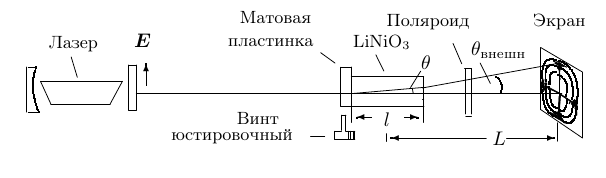
\includegraphics[width=\textwidth]{scheme.png}\label{fig:scheme1}
  \caption{Схема для наблюдения интерференционной картины}
\end{figure}

\begin{figure}[H]
  \centering
  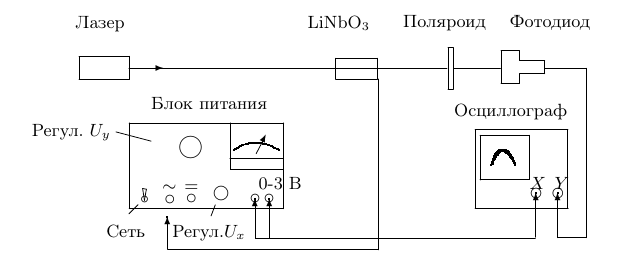
\includegraphics[width=\textwidth]{scheme-2.png}\label{fig:scheme2}
  \caption{Схема для изучения двойного лучепреомления в электрическом поле}
\end{figure}

\section{Работа}
\subsection{Измерение радиусы тёмных колец на экране}
Измерив радиусы тёмных колец на экране получим значения:

\begin{figure}[H]
  \centering
  \begin{tabular}[center]{|c|c|c|c|c|c|c|}
    \hline
    \(\#\)      & 1   & 2   & 3   & 4   & 5   & 6\\\hline
    \(r,\; cm\) & 2.9 & 4.3 & 5.3 & 6.1 & 6.7 & 7.2\\\hline
  \end{tabular}
\end{figure}

Иземерим расстояние \(L\) от серидины кристалла до экрана:
\[ L = 84\;cm \]

\subsection{Определение полуволнового напряжения ниобата лития} \label{sec:U}
Убедимся что направление лазерного луча совпадает с направлением на центр интерференционной картины.

Подключим разъём блока питания на постоянное напряжение, установим регулятор на минимальное
напряжение и включим блок питания в сеть.

Увеличивая напряжение на кристале определим полуволновое напряжение по максимальной яркости пятна на
экране:
\begin{equation} \label{eq:U0.5}
  U_{\lambda/2} = 435\;V
\end{equation}
И по положению следующего минимума - волновое напряжение
\[ U_{\lambda} = U_{\lambda/2} = 960\; V\]

Проделаем всё то же самое для параллельной поляризации лазера и анализатора:
\[ U_{\lambda/2} = 900\;V\]
\[ U_{\lambda} = U_{\lambda/2} = 1440\;V\]

\subsection{Круговая поляризация}
Выставим четвертьволновое напряжение и вращая поляризатор убедимся что свет имеет круговую поляризацию.
(Яркость не изменяется).

\subsection{Фигуры Лиссажу} \label{sec:Liss}
Установим вместо экрана фотодиод (Рис. \ref{fig:scheme2}) и подключим его к \(Y\)-входу осциллографа.
Убрав напряжение до нуля, переключим разъём блока питания на переменное напряжение. С трёхвольтового
выхода БП подадим сигнал на  \(X\)-канал осциллографа. Таким образом, отклонение луча осциллографа по
оси \(X\) будет пропорционально напряжению \(U\) на кристалле, а по оси \(Y\) - интенсивности прошедшего
через анализатор сигнала \(I_{out}\)

Постепенно повышая напряжение на кристалле, будем наблюдать на экране фигуры Лиссажу, соответсвующие
зависимости \(I_{out}\) для скрещенных поляризаций лазера и анализатора. объ1мся от фигуры Лиссажу
симметричности.

\begin{figure}[H]
  \centering
  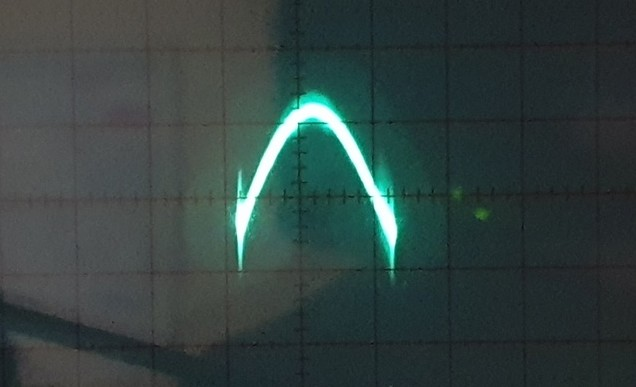
\includegraphics[width=\textwidth]{L1.jpg}\label{fig:L}
  \caption{Фигура Лиссажу}
\end{figure}

Наблюдая за фигурой Лиссажу, определим (по вольтметру на источнике питания) полуволновое напряжение 
\(U_{\lambda/2}\) как \(\Delta U\), соответствующее переходу от макимума к минимуму на осциллограмме.

\[ U_{\lambda/2} = \Delta U = 480 V\]

Это значение довольно точно совпадает со значением \(U_{\lambda/2}\) для поперечной поляризации, полученным
в (\ref{eq:U0.5}).

\subsection{Изменение фигуры Лиссажу}


\begin{figure}[H]
  \centering
  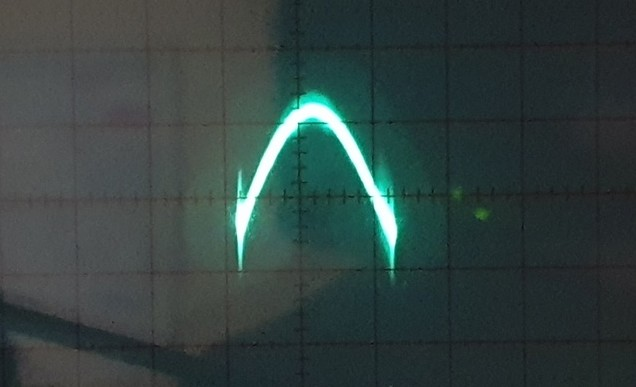
\includegraphics[width=\textwidth]{L1.jpg}\label{fig:L1}
  \caption{Фигура Лиссажу при \(U = U_{\lambda/2}\)}
\end{figure}

\begin{figure}[H]
  \centering
  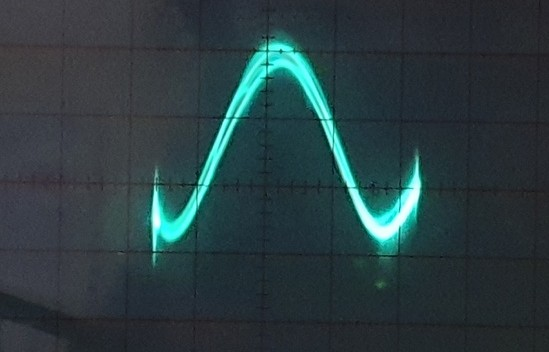
\includegraphics[width=\textwidth]{L2.jpg}\label{fig:L2}
  \caption{Фигура Лиссажу при \(U = U_{\lambda}V\)}
\end{figure}

\begin{figure}[H]
  \centering
  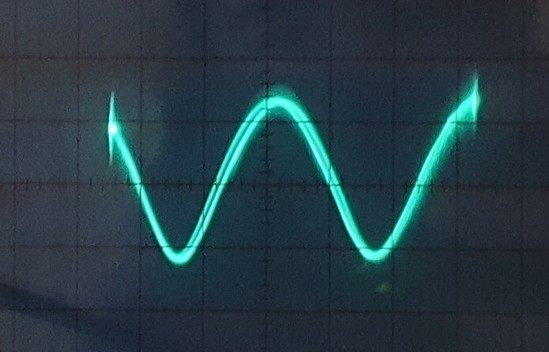
\includegraphics[width=\textwidth]{L3.jpg}\label{fig:L3}
  \caption{Фигура Лиссажу при \(U = U_{3\lambda/2}\)}
\end{figure}

\section{Выводы}
В ходе лабораторной работы:
\begin{enumerate}
  \item Было произведено ознакомление с эффектом Поккельса (Зависимости показателя преломления света в кристалле под действием
  электрического поля и пропорциональности этого изменения от напряжения)
  \item Было измерено полуволновое напряжение для скрещенных поляризаций лазера и поляризатора/анализатора. Полученные значения
  в пунктах: \ref{sec:U} - \(U_{\lambda/2} = 435\;V \) и \ref{sec:Liss} - \(U_{\lambda/2} = 480\;V \) оказались достаточно близки
  и укладываются в приемлимы диапазон (несколько сотен вольт).
\end{enumerate}
\end{document}